% ---- pg-601 （书页 589） ----

\begin{mvtable}
\mvtabcap{表 3\quad $\chi^2$ 分布百分位点}
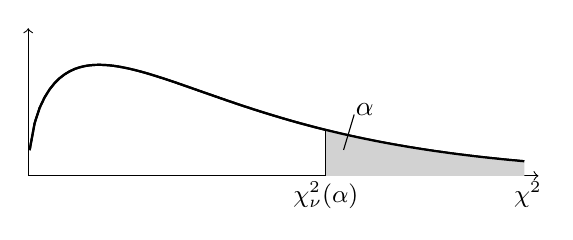
\begin{tikzpicture}[x=0.9cm,y=1.5cm]
% ---- 坐标轴 ----
\draw[->] (0,0) -- (7.2,0);
\draw[->] (0,0) -- (0,1.25);
% ---- 卡方密度曲线（近似） ----
\draw[thick,domain=0.02:7.0,samples=100]
  plot (\x,{1.55*(\x^0.5)*exp(-0.5*\x)});
% ---- 右尾阴影区 ----
\fill[gray!35]
  (4.2,0) -- plot[domain=4.2:7.0,samples=60] (\x,{1.55*(\x^0.5)*exp(-0.5*\x)}) -- (7.0,0) -- cycle;
\draw[thick,domain=0.02:7.0,samples=100]
  plot (\x,{1.55*(\x^0.5)*exp(-0.5*\x)});
% ---- 分位点竖线 ----
\draw (4.2,0) -- (4.2,{1.55*(4.2^0.5)*exp(-0.5*4.2)});
% ---- 标注 ----
\draw (4.6,0.52) -- (4.45,0.22);
\node[inner sep=1pt] at (4.75,0.56) {$\alpha$};
% ---- 轴标签 ----
\node[below,inner sep=1pt,font=\small] at (4.2,-0.02) {$\chi^2_{\nu}(\alpha)$};
\node[below,inner sep=1pt,font=\small] at (7.05,-0.02) {$\chi^2$};
\end{tikzpicture}

{\zihao{6}
\begin{tabular}{r|*{9}{r}}
\toprule
\makecell{d. f.\\$\nu$} & \multicolumn{9}{c}{$\alpha$}\\
\cmidrule(lr){2-10}
& 0.990 & 0.950 & 0.900 & 0.500 & 0.100 & 0.050 & 0.025 & 0.010 & 0.005\\
\midrule
1 & 0.0002 & 0.004 & 0.02 & 0.45 & 2.71 & 3.84 & 5.02 & 6.63 & 7.88\\
2 & 0.02 & 0.10 & 0.21 & 1.39 & 4.61 & 5.99 & 7.38 & 9.21 & 10.60\\
3 & 0.11 & 0.35 & 0.58 & 2.37 & 6.25 & 7.81 & 9.35 & 11.34 & 12.84\\
4 & 0.30 & 0.71 & 1.06 & 3.36 & 7.78 & 9.49 & 11.14 & 13.28 & 14.86\\
5 & 0.55 & 1.15 & 1.61 & 4.35 & 9.24 & 11.07 & 12.83 & 15.09 & 16.75\\
6 & 0.87 & 1.64 & 2.20 & 5.35 & 10.64 & 12.59 & 14.45 & 16.81 & 18.55\\
7 & 1.24 & 2.17 & 2.83 & 6.35 & 12.02 & 14.07 & 16.01 & 18.48 & 20.28\\
8 & 1.65 & 2.73 & 3.49 & 7.34 & 13.36 & 15.51 & 17.53 & 20.09 & 21.95\\
9 & 2.09 & 3.33 & 4.17 & 8.34 & 14.68 & 16.92 & 19.02 & 21.67 & 23.59\\
10 & 2.56 & 3.94 & 4.87 & 9.34 & 15.99 & 18.31 & 20.48 & 23.21 & 25.19\\
11 & 3.05 & 4.57 & 5.58 & 10.34 & 17.28 & 19.68 & 21.92 & 24.72 & 26.76\\
12 & 3.57 & 5.23 & 6.30 & 11.34 & 18.55 & 21.03 & 23.34 & 26.22 & 28.30\\
13 & 4.11 & 5.89 & 7.04 & 12.34 & 19.81 & 22.36 & 24.74 & 27.69 & 29.82\\
14 & 4.66 & 6.57 & 7.79 & 13.34 & 21.06 & 23.68 & 26.12 & 29.14 & 31.32\\
15 & 5.23 & 7.26 & 8.55 & 14.34 & 22.31 & 25.00 & 27.49 & 30.58 & 32.80\\
16 & 5.81 & 7.96 & 9.31 & 15.34 & 23.54 & 26.30 & 28.85 & 32.00 & 34.27\\
17 & 6.41 & 8.67 & 10.09 & 16.34 & 24.77 & 27.59 & 30.19 & 33.41 & 35.72\\
18 & 7.01 & 9.39 & 10.86 & 17.34 & 25.99 & 28.87 & 31.53 & 34.81 & 37.16\\
19 & 7.63 & 10.12 & 11.65 & 18.34 & 27.20 & 30.14 & 32.85 & 36.19 & 38.58\\
20 & 8.26 & 10.85 & 12.44 & 19.34 & 28.41 & 31.41 & 34.17 & 37.57 & 40.00\\
21 & 8.90 & 11.59 & 13.24 & 20.34 & 29.62 & 32.67 & 35.48 & 38.93 & 41.40\\
22 & 9.54 & 12.34 & 14.04 & 21.34 & 30.81 & 33.92 & 36.78 & 40.29 & 42.80\\
23 & 10.20 & 13.09 & 14.85 & 22.34 & 32.01 & 35.17 & 38.08 & 41.64 & 44.18\\
24 & 10.86 & 13.85 & 15.66 & 23.34 & 33.20 & 36.12 & 39.36 & 42.98 & 45.56\\
25 & 11.52 & 14.61 & 16.47 & 24.34 & 34.38 & 37.65 & 40.65 & 44.31 & 46.93\\
26 & 12.20 & 15.38 & 17.29 & 25.34 & 35.56 & 38.89 & 41.92 & 45.64 & 48.29\\
27 & 12.88 & 16.15 & 18.11 & 26.34 & 36.74 & 40.11 & 43.19 & 46.96 & 49.64\\
28 & 13.56 & 16.93 & 18.94 & 27.34 & 37.92 & 41.34 & 44.46 & 48.28 & 50.99\\
29 & 14.26 & 17.71 & 19.77 & 28.34 & 39.09 & 42.56 & 45.72 & 49.59 & 52.34\\
30 & 14.95 & 18.49 & 20.60 & 29.34 & 40.26 & 43.77 & 46.98 & 50.89 & 53.67\\
40 & 22.16 & 26.51 & 29.05 & 39.34 & 51.81 & 55.76 & 59.34 & 63.69 & 66.77\\
50 & 29.71 & 34.76 & 37.69 & 49.33 & 63.17 & 67.50 & 71.42 & 76.15 & 79.49\\
60 & 37.48 & 43.19 & 46.46 & 59.33 & 74.40 & 79.08 & 83.30 & 88.38 & 91.95\\
70 & 45.44 & 51.74 & 55.33 & 69.33 & 85.53 & 90.53 & 95.02 & 100.43 & 104.21\\
80 & 53.54 & 60.39 & 64.28 & 79.33 & 96.58 & 101.88 & 106.63 & 112.33 & 116.32\\
90 & 61.75 & 69.13 & 73.29 & 89.33 & 107.57 & 113.15 & 118.14 & 124.12 & 128.30\\
100 & 70.06 & 77.93 & 82.36 & 99.33 & 118.50 & 124.34 & 129.56 & 135.81 & 140.17\\
\bottomrule
\end{tabular}}
\end{mvtable}
